\documentclass[11pt,oneside,a4paper]{report}

\begin{document}
\section{Types and validation}
The spellchecking equivalent for computer programs could be type checking; the problem of validating a programmers intuition of a program's intent.
Types also have other properties than simply validating they can in fact be related to thorems to which an implementation is the proof~\cite{howard1980formulae}.
\begin{lstlisting}[language=ML,caption={Head implementation},label={lst:headimpl}]
fun head l: List a -> a = 
    match l
        | Cons x _ -> x;
        | Nil -> ?;
    ;
\end{lstlisting}
For instance consider the implementation of type \texttt{List a -> a} in \autoref{lst:headimpl}, a total implementation of the function cannot exist.

The type scheme for the $L$ language will be the Hindley-Milner type system~\cite{hindley1969principal,milner1978theory}.

\subsection{The language of types}
Before delving into types the lambda calculus defined in \autoref{sec:lc} must be agumented with the \textit{let expression} (\autoref{eq:letb}).
\begin{align}
    \texttt{let } x = Y \texttt{ in } E
    \label{eq:letb}
\end{align}
It should be noted that the let binding can be expressed by abstraction and application (\autoref{eq:letaa}).
\begin{align}
    (\lambda x . E) (Y)
    \label{eq:letaa}
\end{align}
The let expression has a nice property that will become apparent later when typing rules are introduced.
The untyped lambda calculus exists at the ``value level'' while the now introduced syntax exists at the ``type level''.
There are two vairants of types in Hindley-Milner, the \textit{monotype} and the \textit{polytype}.
A monotype is either a variable, an abstraction of two monotypes or an application (\autoref{eq:mono}).
\begin{align}
    mono \,\,\tau = a \,|\, \tau \rightarrow \tau \,|\, C \tau_1 \dots \tau_n
    \label{eq:mono}
\end{align}
The application term of the monotype is dependant on the primitive types of the programming language.
In $L$ the set of monotypes are $\{ \texttt{Int}, \texttt{Bool}, \texttt{ADT} \}$.
The types $\tau_1 \dots \tau_n$ are the typevariables required to construct some atomic type.
An instance of which could be a \texttt{List a} wich one type parameter \texttt{a}.
A polytype is a polymorphic type (\autoref{eq:poly}).
\begin{align}
    poly \,\, \sigma = \tau \,|\, \forall a . \sigma
    \label{eq:poly}
\end{align}
A central component of typing in Hindley-Milner is the \textit{environment}.
The environment list $\Gamma$ is a list of pairs of variable and type (\autoref{eq:env}).
$\Gamma \vdash x: \sigma$ implies a \textit{typing judgment} meaning that given $\Gamma$ the variable $x$ has type $\sigma$.
\begin{align}
    \Gamma \,\, = \epsilon \,|\, \Gamma, x : \sigma
    \label{eq:env}
\end{align}

Like in the untyped lambda calculus types also have notions of free and bound type varables.
Varables are bound when they have been introduced by a quantification or exist in the environment set.
\begin{align}
    &free(a) = \{ a \}\\
    &free(C \tau_1 \dots \tau_n ) = \bigcup_{i-1}^n free(\tau_i)\\
    &free(\Gamma) = \bigcup_{x:\sigma \in \Gamma} free(\sigma)\\
    &free(\forall a . \sigma) = free(\sigma) - \{ a \}\\
    &free(\Gamma \vdash x : \sigma) = free(\sigma) - free(\Gamma)
\end{align}

\subsection{Hindley-Milner rules}
With the now introduced primitives the Hindley-Milner type system is but a set of inference rules composed by said primitives.
\begin{figure}[ht]
\begin{mdframed}
    \minipage{0.49\textwidth}
    \begin{prooftree}
        \AxiomC{$x: \sigma \in \Gamma$}
        \LeftLabel{Var}
        \UnaryInfC{$\Gamma\vdash x:\sigma$}
    \end{prooftree}
    \endminipage
    \minipage{0.49\textwidth}
    \begin{prooftree}
        \AxiomC{$\Gamma \vdash e_1 : \tau_1 \rightarrow \tau_2$}
        \LeftLabel{App}
        \AxiomC{$\Gamma \vdash e_2 : \tau_1$}
        \BinaryInfC{$\Gamma \vdash e_1 e_2 : \tau_2$}
    \end{prooftree}
    \endminipage\hfill\vspace{0.8cm}

    \minipage{0.49\textwidth}
    \begin{prooftree}
        \AxiomC{$\Gamma, x: \tau_1 \vdash e : \tau_2$}
        \LeftLabel{Abs}
        \UnaryInfC{$\Gamma \vdash \lambda x . e : \tau_1 \rightarrow \tau_2$}
    \end{prooftree}
    \endminipage\hfill
    \minipage{0.49\textwidth}
    \begin{prooftree}
        \AxiomC{$\Gamma \vdash e_1 : \sigma$}
        \LeftLabel{Let}
        \AxiomC{$\Gamma x : \sigma \vdash e_2 : \tau$}
        \BinaryInfC{$\Gamma \vdash \texttt{ let } x = e_1 \texttt{ in } e_2 : \tau$}
    \end{prooftree}
    \endminipage\hfill\vspace{0.8cm}

    \minipage{0.49\textwidth}
    \begin{prooftree}
        \AxiomC{$\Gamma \vdash e : \sigma_1$}
        \AxiomC{$\sigma_1 \sqsubseteq \sigma_2$}
        \LeftLabel{Ins}
        \BinaryInfC{$\Gamma \vdash e : \sigma_2$}
    \end{prooftree}
    \endminipage\hfill
    \minipage{0.49\textwidth}
    \begin{prooftree}
        \AxiomC{$\Gamma \vdash e : \sigma$}
        \AxiomC{$a \notin free(\Gamma)$}
        \LeftLabel{Gen}
        \BinaryInfC{$\Gamma e : \forall a . \sigma$}
    \end{prooftree}
    \endminipage
\end{mdframed}
\caption{Hindley-Milner type rules}
\label{fig:hmrules}
\end{figure}
There are six rules in the Hindley-Milner rules outlined in \autoref{fig:hmrules}.
The first rule and also the only axiom is the Variable.
The Variable rule states that if some variable $x$ with type $\sigma$ has been deemed to exist, then they must be in the environment.
The Application rule states that if $e_1 e_2$ is of type $\tau_2$ then $e_1$ must conform to a type that can produce a type $\tau_2$ given a type $\tau_1$ and $e_2$ must conform to the type of this $\tau_1$.
The Instatiate rule are important to specify a quantified type $\sigma_1$ to a specific one $\sigma_2$.
Generalization lifts a type into a quantified type for all types which are bound.

\subsection{Damas-Milner Algorithm W}
\begin{figure}[ht]
\begin{mdframed}

    \minipage{0.40\textwidth}
    \begin{prooftree}
        \AxiomC{$x: \sigma \in \Gamma$}
        \AxiomC{$\tau = inst(\sigma)$}
        \LeftLabel{Var}
        \BinaryInfC{$\Gamma \vdash x:\tau , \emptyset$}
    \end{prooftree}
    \endminipage\hfill
    \minipage{0.64\textwidth}
    \begin{prooftree}
        \AxiomC{$\tau_1 = fresh$}
        \AxiomC{$\Gamma, x: \tau_1 \vdash e: \tau_2, S$}
        \LeftLabel{Abs}
        \BinaryInfC{$\Gamma \vdash \lambda x . e : S\tau_1 \rightarrow \tau_2, S$}
    \end{prooftree}
    \endminipage\hfill\vspace{0.8cm}

    \minipage{1\textwidth}
    \begin{prooftree}
        \AxiomC{$\Gamma \vdash e_1 : \tau_1, S_1 \,\,\,\, \tau_3 = fresh$}
        \AxiomC{$S_1 \Gamma \vdash e_2 : \tau_2, S_2 \,\,\,\, S_2 = unify(S_2 \tau_1, \tau_2 \rightarrow \tau_3)$}
        \LeftLabel{App}
        \BinaryInfC{$\Gamma \vdash e_1 e_2 : S_2 \tau_3, S_3 S_2 S_1$}
    \end{prooftree}
    \endminipage\hfill\vspace{0.8cm}

    \minipage{1\textwidth}
        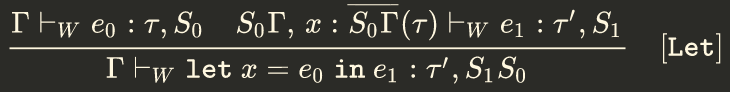
\includegraphics[width=1\textwidth]{let}
    %\begin{prooftree}
        %\AxiomC{$\Gamma \vdash e : \sigma$}
        %\AxiomC{$a \notin free(\Gamma)$}
        %\LeftLabel{Gen}
        %\BinaryInfC{$\Gamma e : \forall a . \sigma$}
    %\end{prooftree}
    \endminipage
\end{mdframed}
\caption{Hindley-Milner type rules}
\label{fig:hmrules}
\end{figure}

\end{document}
